\documentclass[
	%a4paper, % Use A4 paper size
	letterpaper, % Use US letter paper size
]{jdf}

\addbibresource{references.bib}

\author{Shashvat Sinha}
\email{shashvat.sinha@gatech.edu}
\title{Project (Summer 2020)\\CS6750}

\begin{document}
%\lsstyle

\maketitle

\section{Introduction}
\subsection{Interface Description}
The interface we have chosen to redesign is the on-screen keyboard for Xbox One consoles. This interface shows up whenever a user has to type in characters from a keyboard into a textbox. It is used for searching, username and password input and the Xbox Live short message service. The keyboard made its appearance with the release of the Xbox One in November 2013.

\begin{figure}[h]
	\centering
	\frame{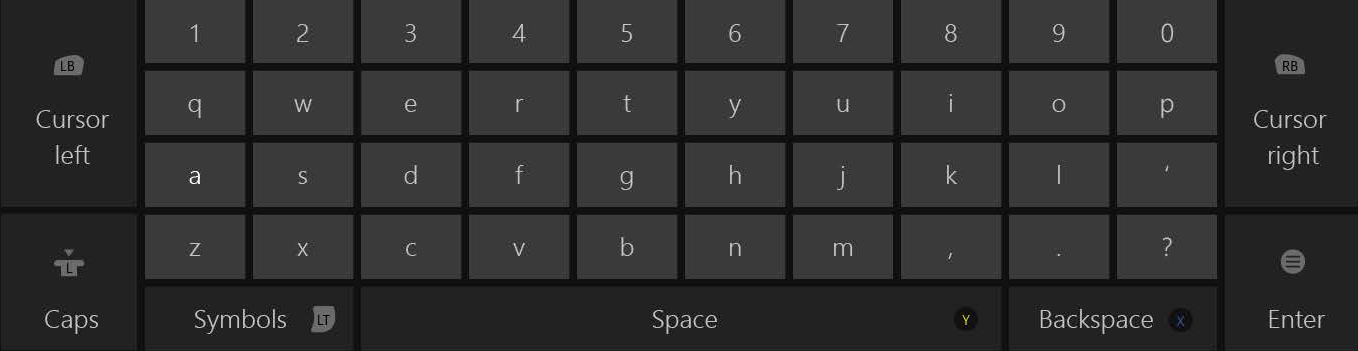
\includegraphics[width=14cm]{jdf-master/Figures/xbox-one-virtual-keyboard.jpg}}
	\caption{Xbox One Virtual Keyboard}
	\label{fig:xb1keyboard}
\end{figure}


A detailed description of the keyboard design is given on the portfolio page of the designer, Matthew Hartman (\cite{hartman_2013}).


In order to use the keyboard, one must have an Xbox One console. On the console, navigate to any screen that requires textual input, for example the search box on the Microsoft Store page, or the password input page on the wireless network configuration screen. This should bring up the keyboard on screen.

\begin{figure}[h]
	\centering
	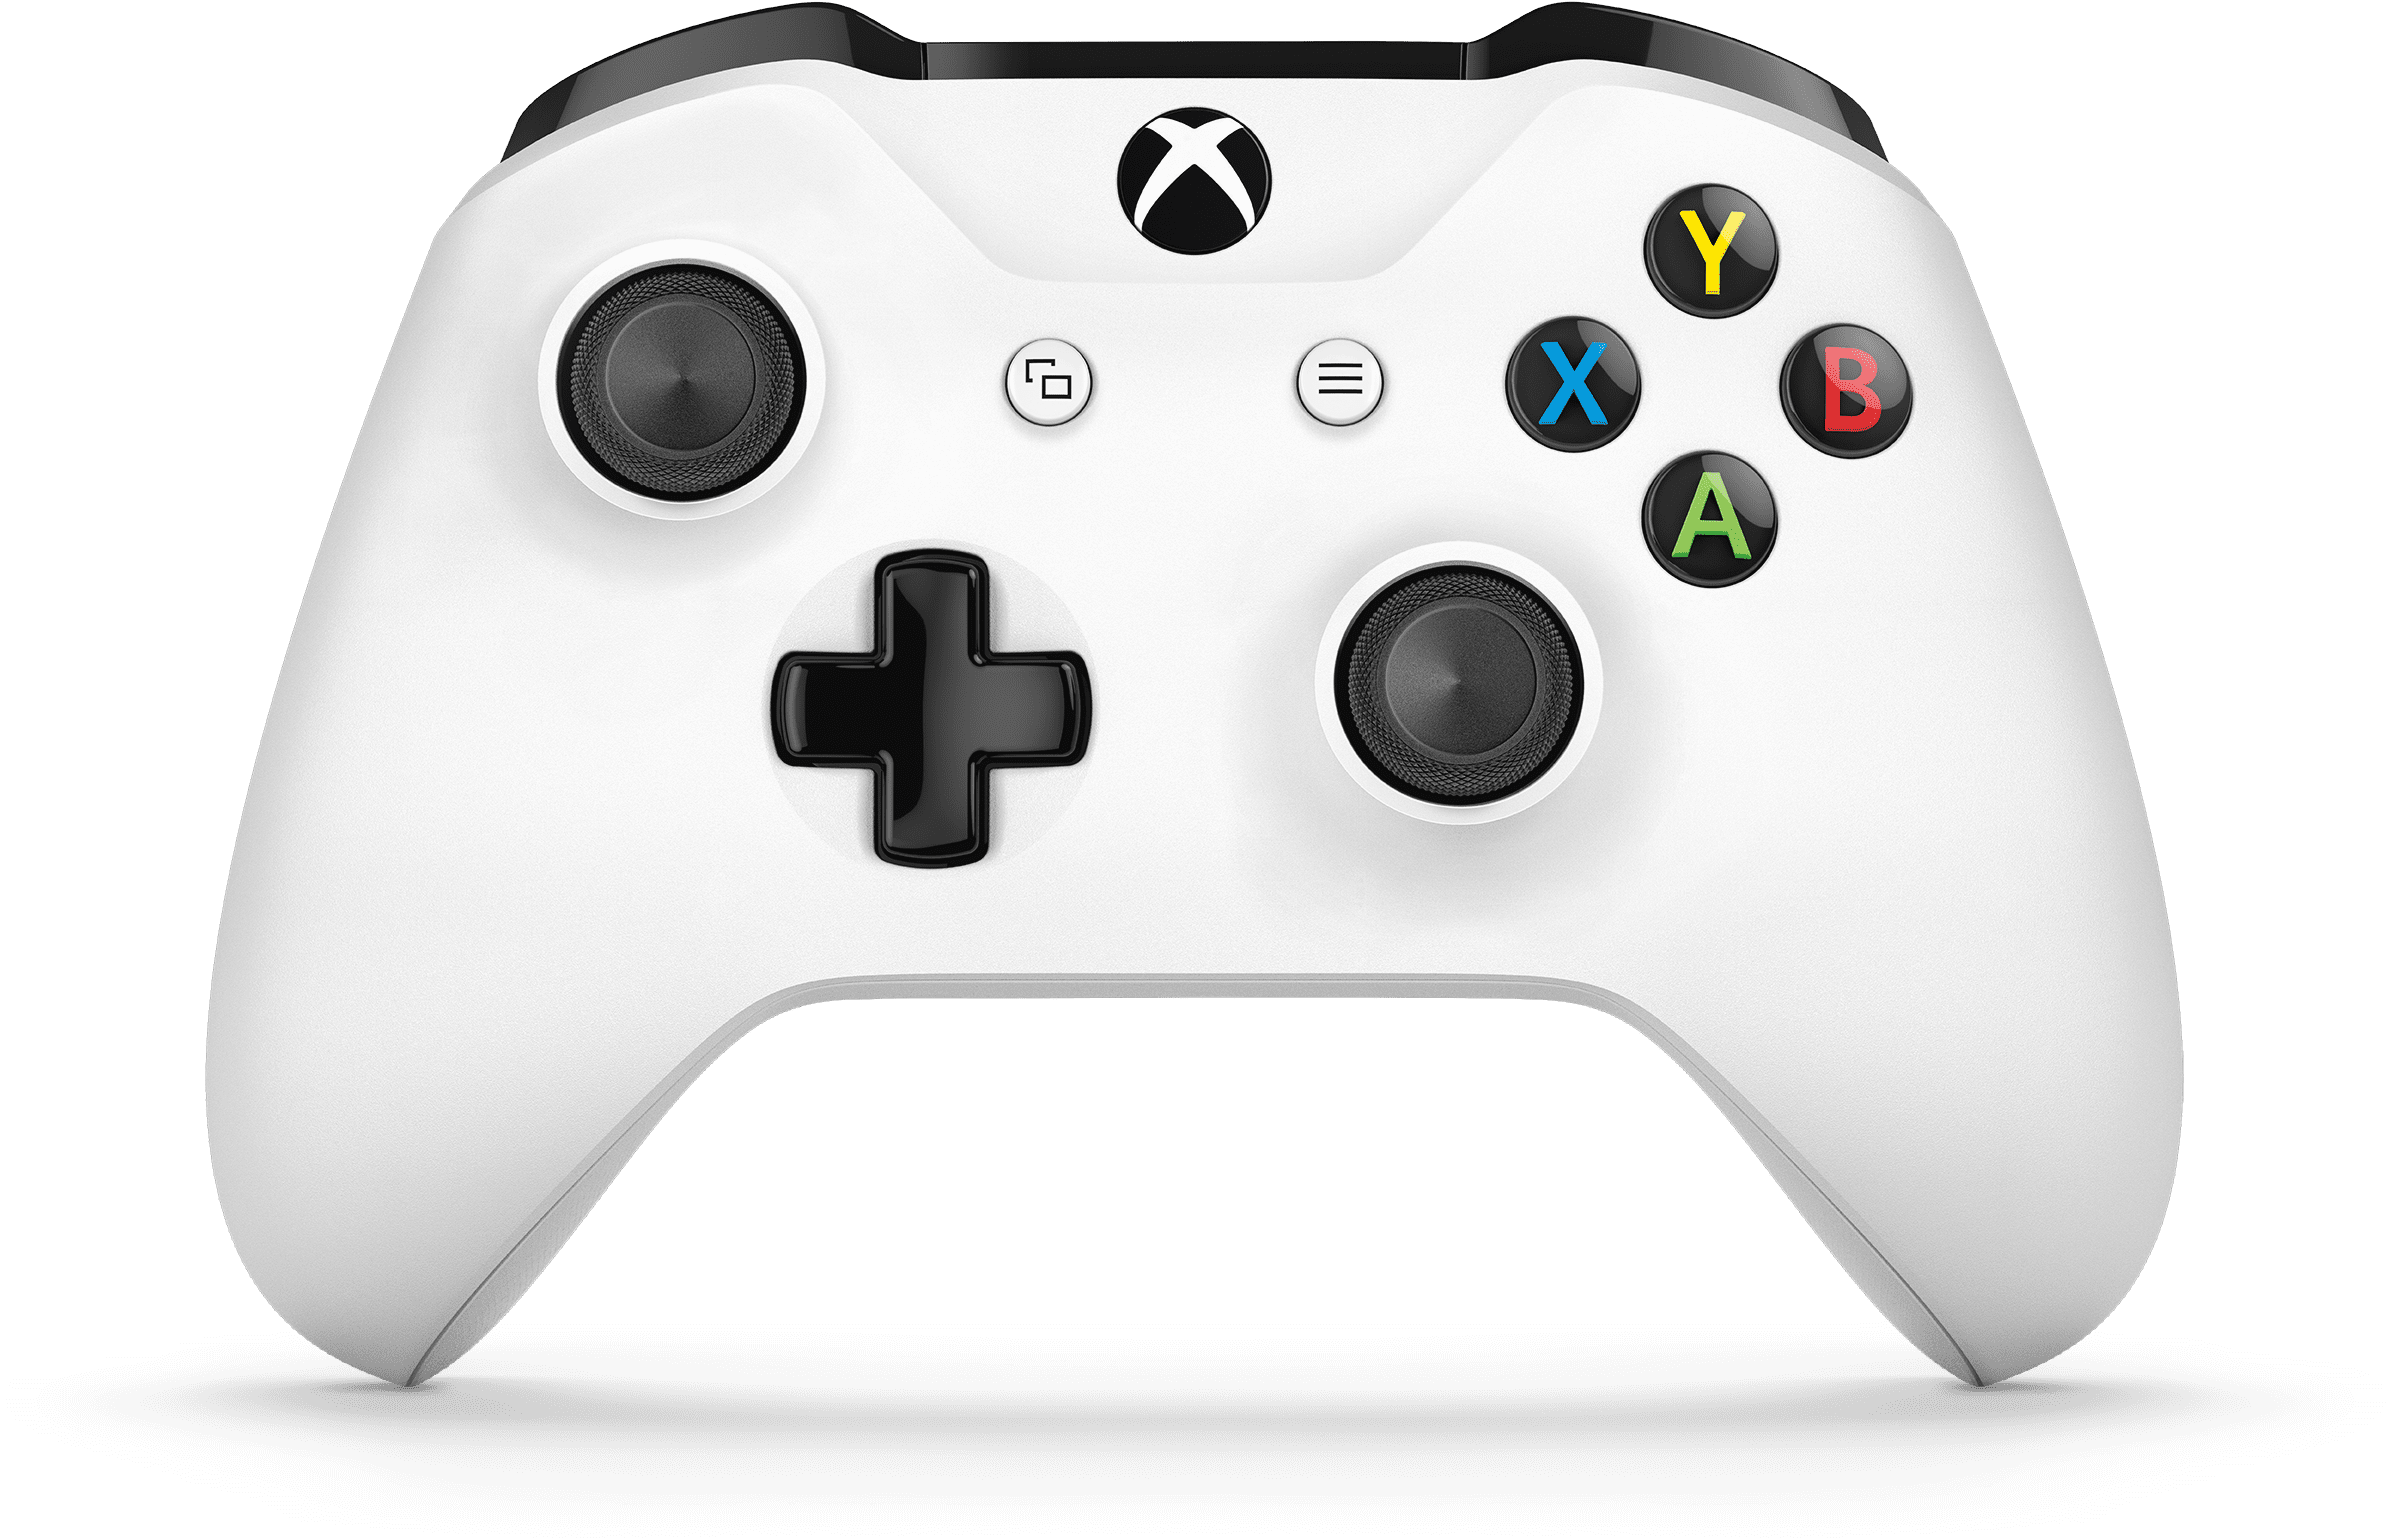
\includegraphics[width=10cm]{jdf-master/Figures/xbox-one-controller.png}
	\caption{Xbox One Controller}
	\label{fig:xb1controller}
\end{figure}

The keyboard is operated by the Xbox controller, a handheld device that has a variety of physical inputs on it - two sticks that can be moved in circular directions (thumbsticks), four colored buttons A, B, X \& Y, four directional buttons (cursor keypad), two buttons under the left and right trigger fingers (left and right triggers) and two buttons above the triggers (left and right shoulder buttons). The controller is also equipped with haptic feedback for the triggers and also general vibration. And last but not the least, the thumbsticks are also buttons, operated by pressing them axially.

The keyboard is operated by utilizing the Xbox controller to select letters to be typed, then pressing a button to select that letter. This is done one letter at a time.

\subsection{Scope}
We will not be redesigning the controller. We will only be redesigning the onscreen virtual keyboard, and the interaction of the controller with the virtual keyboard.

\section{Initial Needfinding}
\subsection{Choice of Needfinding Type}
For our initial needfinding, we will use publicly available data in the form of product reviews, opinion pages, design patents (wherein they identify particular problems they are trying to solve), scholarly papers and so on.

Our objective is to determine what are the shortcomings with the existing virtual keyboard interface on-screen of the Xbox One. 

\subsection{Needfinding Approach}
The volume of literature on the Xbox virtual QWERTY keyboard is not large by any means. So we will divide our needfinding into two parts:
\begin{itemize}
    \item Research on QWERTY keyboards, focusing on virtual/on-screen implementations.
    \item Research on game controllers input/selection techniques.
\end{itemize}

We will use Google Scholar (\url{https://scholar.google.com}) to find articles of interest. We will also use generic searches on Google search to find articles of interest.

In those articles we will search for critiques of QWERTY keyboards, find any quantitative or emperical studies performed and the results thereof.

We will also review papers and articles on methods of input using game controllers that can inform us on better approaches towards using the Xbox One Game controller for input.

\subsection{Needfinding Execution}
\subsubsection{Findings on QWERTY Keyboards}
The QWERTY keyboard was designed during the second half of the 19th century by Sholes et. al (\cite{sholes_glidden_soule_1868}) as a means of writing by type. The primiary consideration during its design was the ability of the rudimentary mechanical devices of those days to be able to function properly with the demands of typing in the English language i.e. not get jammed. There is however, a secondary reason for the layout of the keyboard in the QWERTY form, and not ABCDE form, and that was to do with the needs of the original users of the typewriter - telegraph operators (\cite{stamp_2013}), who needed a device that was well suited to transcribing Morse Code into English. It can be seen that Sholes et. al. did actually follow needfinding approaches for their HMI (human-machine-interface) product development and listened to the needs of their users, contrary to popular belief. This section of research was established the original design context of the QWERTY keyboard. That context does not exist now, and needs to be updated.

Multiple forms of research have been performed on QWERTY keyboards with critical analysis done and alternatives proposed - 

In "\textit{The design and evaluation of a high-performance soft keyboard}" (\cite{mackenzie_zhang_1999}) we see that QWERTY as a keyboard layout lags in performance when compared to other virtual keyboard types. Mackenzie and Zhang employ Fitts's Law to quantitatively model an ideal keyboard layout, which they called Opti, that had a 35\% better performance than the standard QWERTY layout - in a virtual keyboard setting.

In "\textit{Performance Optimization of Virtual Keyboards}" (\cite{zhai_hunter_smith_2002}) we see that an optimally designed Hooke keyboard has 48\% improvement in words per minute (wpm) efficiency over QWERTY while the further optimized Metropolis approach gets to 42.5 wpm movement efficiency, which was 50\% higher than Qwerty and 10\% higher than OPTI.

In \textit{"Efficient keyboard layouts for sequential access in augmentative and alternative communication"} (\cite{venkatagiri_1999}) we see that rowscanning for QWERTY keyboard layouts is far more inefficient than row-column scanning, i.e. even within QWERTY approaches, there are possibilities for optimisation.

\subsubsection{Findings on Game Controller Input}
Our objective here is to see how thumbsticks can be best employed for user input.

In \textit{"TwoStick: Writing with a Game Controller"} (\cite{twostick_2007}) we see a method for typing that uses the standard QWERTY keyboard but utilizes both thumbsticks rather than just one, for improved speed and accuracy.

\begin{figure}[h]
	\centering
	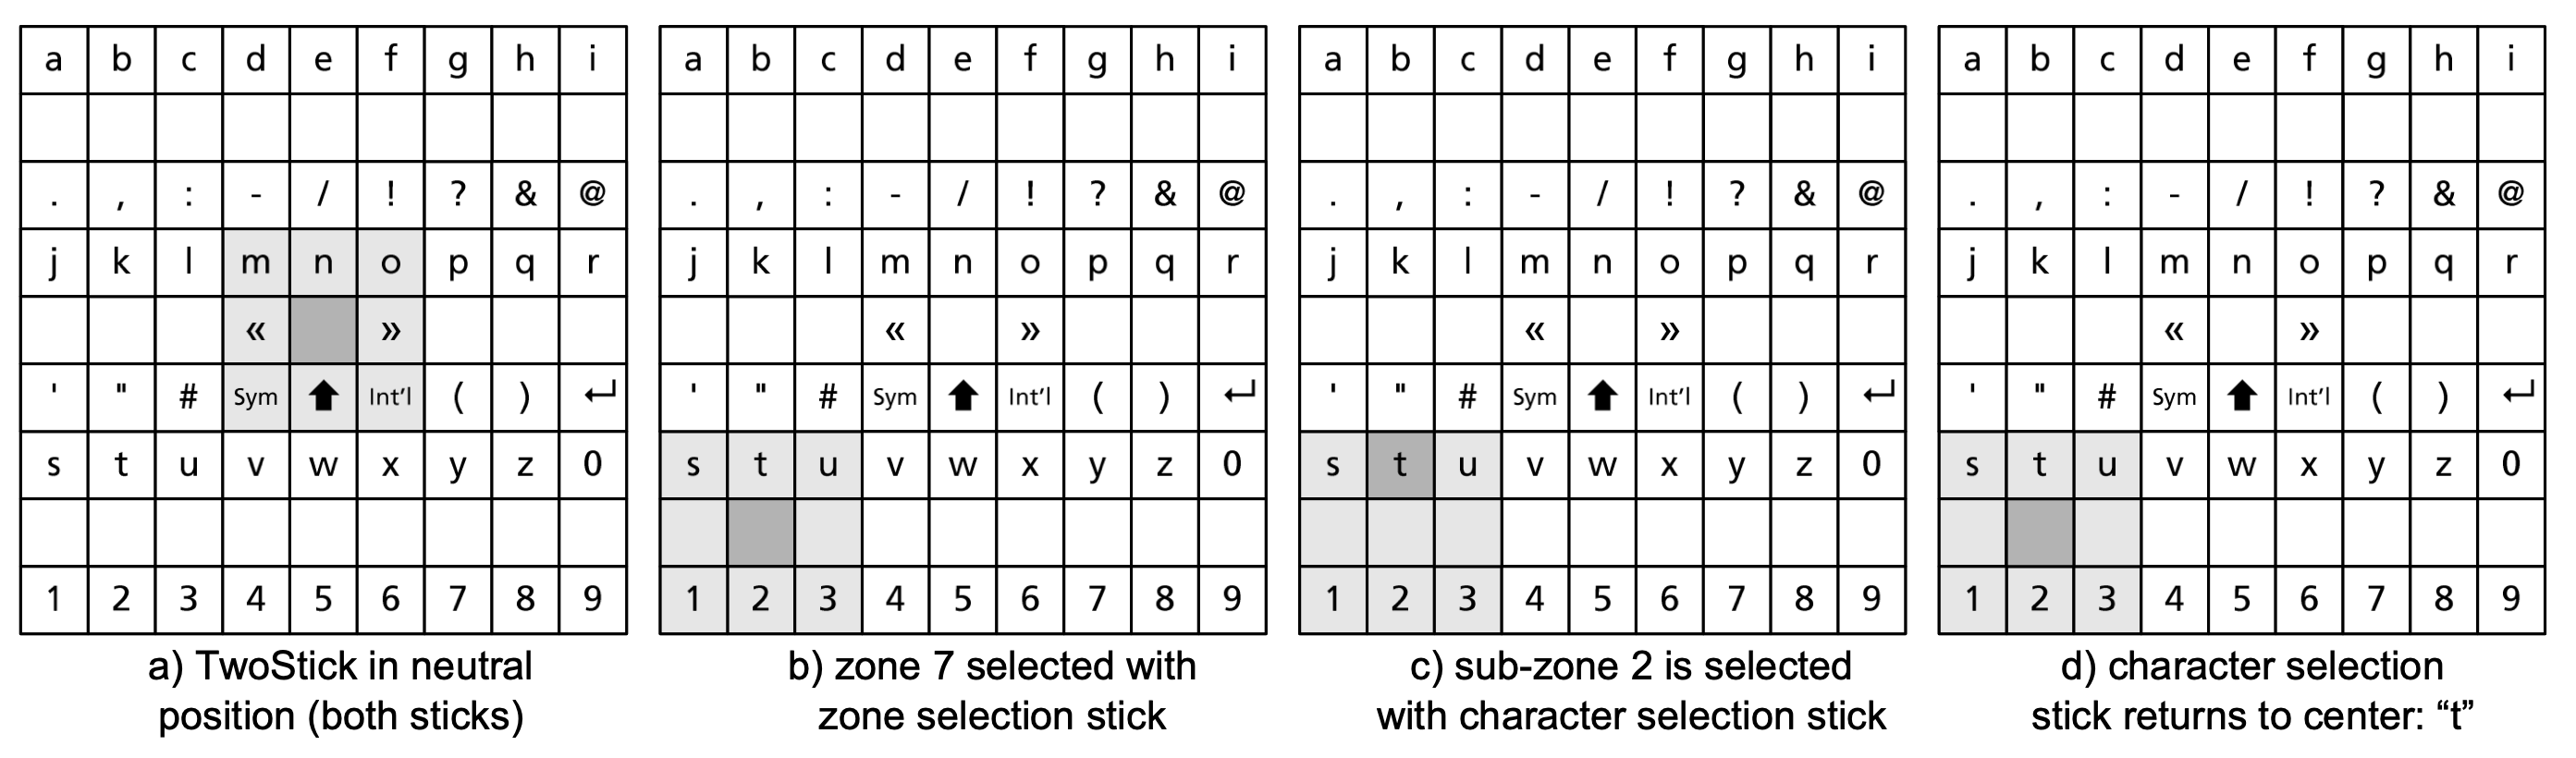
\includegraphics[width=14cm]{jdf-master/Figures/twostick.png}
	\caption{TwoStick Text Entry}
	\label{fig:twostick}
\end{figure}

In \textit{"Text Entry Using a Dual Joystick Game Controller"} (\cite{wilson_agrawala_2006}) the authors employ a dual-QWERTY layout with the left thumbstick selecting letters on the left side of an onscreen QWERTY keyboard and the right thumbstick selecting from the right. Here they saw a statistically significant difference between single-stick and double-stick input.

The patent \textit{"Graphic user interface for a digital content delivery system using circular menus"} \cite{eatsy_taplin_chechik_nelson_2002}) shows how a circular layout can be used to select menu items. 

\begin{figure}[h]
	\centering
	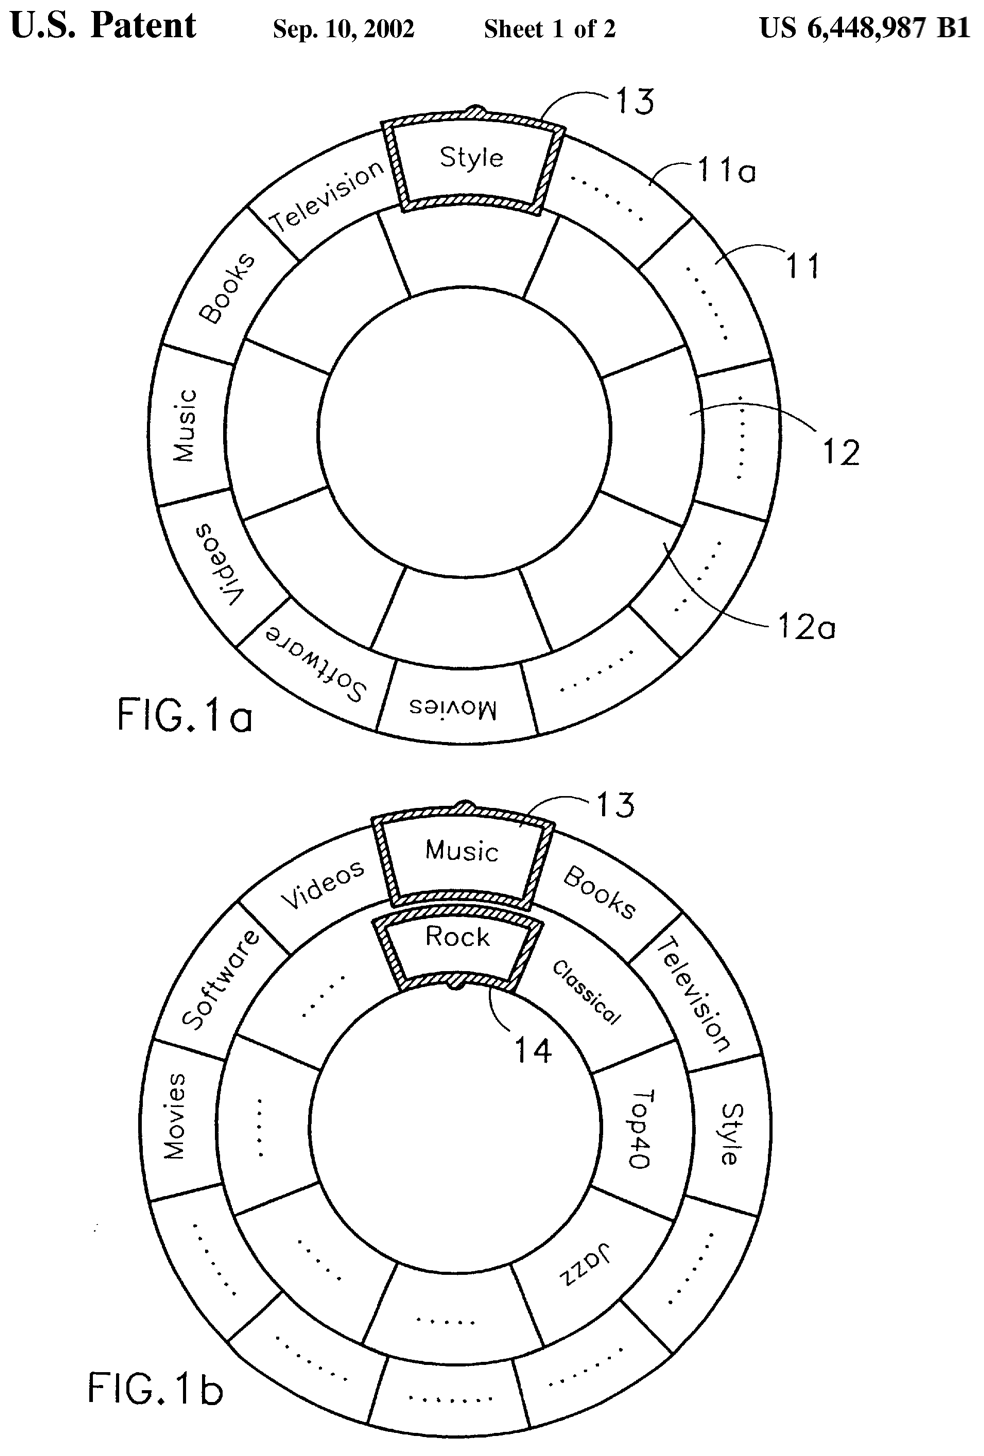
\includegraphics[width=5cm]{jdf-master/Figures/circularmenu.png}
	\caption{Circular Menus}
	\label{fig:circularmanu}
\end{figure}

\subsubsection{Conclusions}
We would make the following three conclusions from our research:
\begin{enumerate}
    \item The QWERTY keyboard layout has had sufficient research done on it to demonstrate that alternative approaches are better. However despite that, the QWERTY layout continues to be the preferred layout.
    \item Even when restricting ourselves to QWERTY layouts, it is possible to improve text input speed and accuracy by using both thumbsticks as inputs.
    \item Thumsticks rotate in the circular domain and therefore lend themselves better to a circular layout of menu items. Note that this approach now has mainstream acceptance in games such as Grand Theft Auto V and Star Wars Battlefront.
\end{enumerate}


We see that such circular entry approaches have now become mainstream in multiple console video games such as Call of Duty, Battlefront and Grand Theft Auto V.



\section{Heuristic Evaluation}

\section{Interface Redesign}

\section{Interface Justification}

\section{Evaluation Plan}


\section{References}

\printbibliography[heading=none]


\end{document}